%! TeX program = lualatex
%tags! hakimi handshaking graphs chapter 1

\documentclass[letterpaper]{article}
\usepackage[margin=1.4in]{geometry}
\usepackage{amsmath}
\usepackage{amssymb}
% \usepackage[macchiato, textcolor=true, pagecolor=true]{catppuccinpalette}
\usepackage[no-math]{fontspec}
\usepackage[fg,bg]{gruvboxpalette}
\usepackage{hyperref}
\usepackage{newtxsf}
% \usepackage{varwidth}
\usepackage[explicit]{titlesec}
\usepackage{tikz}
\usepackage[most]{tcolorbox}
\usetikzlibrary{calc}
\usetikzlibrary{positioning}
\usetikzlibrary{arrows.meta}
\usepackage{tabularray}
\DefTblrTemplate{firsthead, middlehead,lasthead}{default}{}
\DefTblrTemplate{capcont}{default}{}
\DefTblrTemplate{contfoot-text}{normal}{} \SetTblrTemplate{contfoot-text}{normal} \DefTblrTemplate{conthead-text}{normal}{} \SetTblrTemplate{conthead-text}{normal}
\UseTblrLibrary{counter}
\hypersetup{
  colorlinks  = true,
  urlcolor    = CtpBlue,
  linkcolor   = CtpBlue,
  citecolor   = CtpBlue
}
\usepackage[most]{tcolorbox}

\setmainfont{NotoSans-Regular}[
Path           = /home/snouflake/.fonts/ ,
Extension      = .ttf ,
BoldFont       = NotoSans-Bold ,
ItalicFont     = NotoSans-Italic ,
BoldItalicFont = NotoSans-BoldItalic,
] 
\setlength\parindent{0pt}

\usepackage{mathastext}

\def \T {Graph Theory and Modeling}
\def \S {Chapter 1: Basic Notions of Graphs}

\tikzset{
  defaultNode/.style={%
    circle, minimum size=8pt, draw,
  }
}

\begin{document}
\begin{tikzpicture}
  \node[circle, minimum size=12pt, fill=blue, draw]
    (dot1) at (0.8,1) {};
  \node[circle, minimum size=12pt, fill=green, draw]
    (dot2) at (0,0.4) {};
  \node[circle, minimum size=12pt, fill=aqua, draw]
    (dot3) at (0.6,-0.2) {};
  \draw[thick,>=latex,->] 
    (dot1) edge[bend right] (dot2.north)
    (dot3) edge[bend right] (dot2.east)
    (dot2) edge[bend right] (dot3)
    ;
  \node[anchor=west] (titlepicture) at (1.3,0.4) { 
      \begin{tikzpicture}
        \node[anchor=west] 
        (title) at (0,0.9) {\Huge\bfseries\T};
        \node[anchor=west] 
        (subtitle) at (0,0) {\Large\bfseries\S};
      \end{tikzpicture}
    }
    ;
\end{tikzpicture}

\section*{Basic Terms}
\vspace{-1cm}

\begin{longtblr}{
    colspec={@{}Q[3cm,cmd=\textbf] X@{}},
    rowsep={7pt}
  }
  Graph
  & A graph is defined as a pair of sets: $(V, E)$, where $V$ is the set of nodes (vertices) and $E$ is a set of pairs of members of $V$ (edges). If the graph is directed, the edges are also known as arcs. An arc $(v,u)$ is said to have a tail end at $v$ and a head end at $v$. When $\exists$ an edge between nodes they are called adjacent.
  \\
  Loop
  & An edge $(u,u)$ for some $u \in V$ \hspace{5mm}
  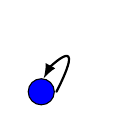
\begin{tikzpicture}[baseline=0mm]
    \node[defaultNode, fill=blue, ]
    (dot1) at (0,0) {};
    \draw[thick,>=latex,->,line cap=round] ($(dot1.east) + (0.02,0)$) .. controls (0.6,0.8) and (0.1,0.3) .. (dot1.80)
    ;
  \end{tikzpicture}
  \\
  Simple Graph
  & A graph without loops
  \\
  Subadjacent graph
  & 
  {
    Let $G = (V,E)$ be a directed graph. Its subadjacent graph $\bar{G}$ is an undirected graph that has an edge $(u,v)$ for every arc $(u,v)$. In the case of $G$ having arcs $(u,v)$ and $(v,u)$, both are replaced by a single edge $(u,v)$.

    \begin{minipage}[t]{\linewidth}
      \begin{center}
        \begin{tikzpicture}[]
          \node[anchor=east] (graph1) at (0,0) {%
              \begin{tikzpicture}
                \node[defaultNode, fill=blue, ]
                  (dot1) at (0.4,0.7) {};
                \node[defaultNode, fill=blue, ]
                  (dot2) at (0,0) {};
                \node[defaultNode, fill=blue, ]
                  (dot3) at (0.8,0) {};
                \draw[thick,>=latex,->,line cap=round] 
                  (dot1) edge[bend right] (dot2)
                  ;
                \draw[thick,>=latex,->,line cap=round] 
                  (dot2) edge[bend right] (dot3)
                  ;
                \draw[thick,>=latex,->,line cap=round] 
                  (dot3) edge[bend right] (dot1)
                  ;
                \draw[thick,>=latex,->,line cap=round] 
                  (dot1) edge[bend right] (dot3)
                  ;
              \end{tikzpicture}
            };

            \node[anchor=center] (to) at (1,0) {\LARGE$\to$};
            \node[anchor=west] (graph2) at (2,0) {%
              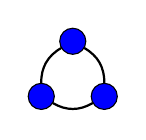
\begin{tikzpicture}
                \node[defaultNode, fill=blue, ]
                  (dot1) at (0.4,0.7) {};
                \node[defaultNode, fill=blue, ]
                  (dot2) at (0,0) {};
                \node[defaultNode, fill=blue, ]
                  (dot3) at (0.8,0) {};
                \draw[thick,>=latex,line cap=round] 
                  (dot1) edge[bend right] (dot2)
                  ;
                \draw[thick,>=latex,line cap=round] 
                  (dot2) edge[bend right] (dot3)
                  ;
                \draw[thick,>=latex,line cap=round] 
                  (dot3) edge[bend right] (dot1)
                  ;
              \end{tikzpicture}
            };
          \end{tikzpicture}
\end{center}
\end{minipage}
  }
  \\
  Trail
  & A succession (node, edge, node, edge, ...)
  \\
  {Circuit \\ (Closed Trail)}
  & A trail in which the first and last nodes are the same.
  \\
  Path
  & A trail where all nodes are distinct
  \\
  {Cycle \\ (Simple circuit)}
  & A circuit in which all nodes but the first and last are distinct.
  \\
  Length
  & The number of edges in a trail
  \\
  Power Set
  & The power set $\mathcal{P}(S)$ is the set of all subsets of $S$, including $S$
  \\
  Adjacency Function
  & {
    Let $G = (V,E)$ the adjacency function $\Gamma$ is defined:

    \begin{math}
      \Gamma(u): V \to \mathcal{P}(V) = \{v \in V: (u,v) \in E\} \forall u \in V 
    \end{math}
  }
  \\
  Adjacency Matrix
  & {Let $G = (V,E) ~s.t.~ V = \{v_1, v_2,\dots,v_n\}$. The adjacency matrix $A$ is a square matrix of size $n \times n$ such that $\forall a_{ij}, a_{ij} = \left\{
    \begin{array}{ll}
      1 & (v_i, v_j) \in V \\
      0 & (v_i, v_j) \notin V \\
    \end{array}
  \right.$
  }
  \\
  {Grade \\ (not directed)}
  & {
    The grade of a node $v$, $d(v)$ is the number of edges that are incident with it. *A loop adds two units to the grade, not one.
    \medskip

    If the grade of a node is 0, it is called isolated.
    \medskip
    
    The maximum degree of a graph $G$ is written $\Delta(G)$, while the minimum is written $\delta(G)$.
  }
  \\
  {Grade \\ (directed)}
  & {
    The indegree of a node v, $d^-(v)$, is the number of edge head ends adjacent to it.
    \medskip

    The outdegree, $d^-(v)$, conversely, is the number of edge tail ends adjacent to it.
  }
  \\
  {
    Obtaining degree from adjacency matrix
  }
  & {
    The degree of a node $i$ from an undirected graph can be obtained by summing either the column or row $i$ of the graph's adjacency matrix, and adding 1 if the node has a loop.
    \medskip

    If the graph is directed, the outdegree can be obtained by summing the row $i$ and the indegree can be obtained by summing the column $i$.
  }
  \\
  Handshaking Lemma
  & {
    Let $G = (V,E)$ be an undirected graph. $\sum_{v \in V} d(v) = 2\#E$.
    \medskip

    $\therefore$ the number of nodes with an uneven grade is even.
    \medskip

    Let $G$ be now be a directed graph. $\sum_{v \in V} d^+(v) = \sum_{v \in V} d^-(v) = \#E$
  }
\end{longtblr}

\section*{Subgraphs}
Let $G$ and $H$ be graphs.

\vspace{-1cm}
\medskip

\begin{longtblr}{
    colspec={@{}Q[3cm,cmd=\textbf] X@{}},
    rowsep={7pt}
  }
  Subgraph
  & {
    $H$ is a subgraph of $G$ $\iff V(H) \subset V(G) \land E(H) \subset E(G)$
  }
  \\
  Spanning Subgraph
  & $H$ is a spanning subgraph of $G$ $\iff$ $H$ is a subgraph of $G$ $\land~ V(H) = V(G)$
  \\
  Induced subgraph
  & {
    $H$ is a subgraph of $G$ induced by $E'$ ($H = G[E']$) for some 
    $E' \subset E(G)$ $\iff E(H) = E' \land V(H) = \{v \in V(G): v \text{ is and endpoint of some } e \in E\}$
    \medskip

    $H$ is a subgraph of $G$ induced by $V'$ ($H = G[V']$) for some 
    $V' \subset V(G)$ $\iff V(H) = V' \land E(H) = \{e \in E: \text{the endpoints of e}\}$
  }
  \\
  Subtraction
  & {
    Let $V' \subset V(G)$, $E' \subset E(G)$.

    \begin{minipage}[t]{\linewidth}
      \begin{itemize}
        \item 
          $G - V' = (V - V', R - \{e \in E: e_1 \in V' \lor e_2 \in V'\})$
        \item
          $G - E' = (V, E - E')$
        \item
          Let $e \in E'$. $G - e = G - \{e\}$
      \end{itemize}
    \end{minipage}

  }
\end{longtblr}

\section*{Graphic Sequences}

\vspace{-1cm}
\begin{longtblr}{
    colspec={@{}Q[3cm,cmd=\textbf] X@{}},
    rowsep={7pt}
  }
  Graphic Sequence
  & A sequence of integers is considered a graphic sequence $\iff$ there exists an undirected graph such that the values of the sequence correspond to the degrees of its nodes.
  \\
  Harvel-Hakimi Theorem
  & {Let the following be a sequence of decreasing integers: $(s, t_1, t_2, \dots, t_s, d_1, d_2, \dots, d_r)$.
    $(s, t_1, t_2, \dots, t_s, d_1, d_2, \dots, d_r)$ is a graphic sequence $\iff$ $(t_1 - 1, t_2 - 1, \dots, t_s - 1, d_1, d_2, \dots, d_r)$ is also a graphic sequence.
    \medskip

    \begin{minipage}[t]{\linewidth}
      \begin{tcolorbox}[%
        nobeforeafter,
        enhanced,
        top=3mm,
        attach boxed title to top left={xshift=3mm,yshift=-3mm},
        boxed title style={colback=font!10!background,colframe=font},
        before title=\bfseries,
        coltitle=font,
        colback=font!10!background,
        colframe=font,
        title={Hakimi's Algorithm}
        ]
        Let $S$ be a decreasing sequence of integers: $(d_1, d_2, \dots, d_n)$.
        \medskip

        $(\sum_{i=1}^{n} d_i \text{ is odd } \lor d_1 > n - 1) \Rightarrow$ S is not a graphic sequence.

        \begin{tikzpicture}[%
          draw=font!90!background,
          text=font!100!background,
          ]
          \node (margin) at (0,0) {};
          \node (sum) at (7,-0.2) {\tiny Breaks the Handshaking Lemma};
          \draw[>=latex]
            (sum.west) edge[bend left=10,->] (1,0);
          \node (size) at (7,-0.5) {\tiny The sequence has too few nodes};
          \draw[>=latex]
            (size.west) edge[bend left=10,->] (3.5,0);
        \end{tikzpicture}
        \medskip


        \begin{tikzpicture}[%
          node distance=1pt,
          mtext/.style={anchor=west,inner sep=0pt,line width=0pt},
          ttext/.style={anchor=north west,inner sep=0pt,line width=0pt,text width=5cm,font=\footnotesize},
          solvedNode/.style={defaultNode,minimum size=2pt,inner sep=2pt,fill=blue,anchor=center}
          ]
          \node[mtext,anchor=center] (initS) at (0,0) {\strut$S$};
          \node[mtext] (initEq) at (initS.east) {\strut$\,=\,$};


          \foreach \x [count=\xi,remember=\xi as \prevxi] in {3,3,2,1,1,0}
          {
            \ifnum \xi < 2
              \node[mtext] (initSeq\xi) at (initEq.east) {\strut$(\x,$};
            \else
              \node[mtext] (initSeq\xi)  at (initSeq\prevxi.east) {\strut$\x$\ifnum\xi>5$)$\else$,$\fi};
            \fi
          }

          \node[solvedNode] (t1n1) at (0,-2.6em) {$3$};

          \node[mtext] (otherwise) at ($(t1n1.west) + (0,5.2em)$) {Otherwise:\strut};

          \draw[>=latex,thick,blue] (initSeq1.south) edge[->,bend left=20] (t1n1.50);

          \foreach \x [count=\xi,remember=\xi as \prevxi] in {3,2,1,1,0}
          {
            \ifnum \xi < 2
              \node[mtext] (t1initSeq\xi) at (initSeq1.west |- t1n1) {\strut$(\x,$};
            \else
              \node[mtext] (t1initSeq\xi)  at (t1initSeq\prevxi.east) {\strut$\x$\ifnum\xi>4$)$\else$,$\fi};
            \fi
          }

          \node[solvedNode] (t1n2) at (0,-5.2em) {0};

          \foreach \x [count=\xi,remember=\xi as \prevxi] in {2,1,0,1,0}
          {
            \ifnum \xi < 2
              \node[mtext] (t1less\xi) at (initSeq1.west |- t1n2) {\strut$(\x,$};
            \else
              \node[mtext] (t1less\xi) at (t1less\prevxi.east) {\strut$\x$\ifnum\xi>4$)$\else$,$\fi};
            \fi

            \ifnum \xi < 4
              \draw (t1n2.south) edge[bend right=40] node[rectangle,fill=font!10!background,inner sep=0,near end]{\tiny$-1$} (t1less\xi.south);
            \fi
          }

          \node[solvedNode] (t1n3) at (0,-7.8em) {0};

          \foreach \x [count=\xi,remember=\xi as \prevxi] in {2,1,1,0,0}
          {
            \ifnum \xi < 2
              \node[mtext] (t1Sorted\xi) at (initSeq1.west |- t1n3) {\strut$(\x,$};
            \else
              \node[mtext] (t1Sorted\xi) at (t1Sorted\prevxi.east) {\strut$\x$\ifnum\xi>4$)$\else$,$\fi};
            \fi
          }

          \draw
            (t1n3) edge[bend right=40] (t1Sorted1.south)
            (t1n3) edge[bend right=40] (t1Sorted2.south)
            (t1n3) edge[bend right=30] (t1Sorted4.south)
            ;
          \draw[]
            (t1Sorted3.north) edge[bend left=50,{Latex[length=0.8mm, width=0.8mm]}-{Latex[length=0.8mm, width=0.8mm]}] (t1Sorted4.north);
            ;

          \node[solvedNode] (t1n4) at (0,-10.4em) {0};
          \node[solvedNode,right=3pt of t1n4,fill=aqua] (t2n1)  {2};
          \draw[>=latex,thick,aqua] (t1Sorted1.south) edge[->] (t2n1.north);

          \foreach \x [count=\xi,remember=\xi as \prevxi] in {1,1,0,0}
          {
            \ifnum \xi < 2
              \node[mtext,right=3pt of t2n1] (t2initSeq\xi) {\strut$(\x,$};
            \else
              \node[mtext] (t2initSeq\xi) at (t2initSeq\prevxi.east) {\strut$\x$\ifnum\xi>3$)$\else$,$\fi};
            \fi
          }
          
          \draw
            (t1n4) edge[bend right=40] (t2initSeq1.south)
            (t1n4) edge[bend right=30] (t2initSeq3.south)
            (t1n4) edge[bend right=40] (t2n1.south);

          \node[solvedNode] (t1n5) at (0,-13.0em) {0};
          \node[solvedNode,right=3pt of t1n5,fill=aqua] (t2n2)  {0};

          \foreach \x [count=\xi,remember=\xi as \prevxi] in {0,0,0,0}
          {
            \ifnum \xi < 2
              \node[mtext,right=3pt of t2n2] (t2initSeq\xi) {\strut$(\x,$};
            \else
              \node[mtext] (t2initSeq\xi) at (t2initSeq\prevxi.east) {\strut$\x$\ifnum\xi>3$)$\else$,$\fi};
            \fi
          }
          
          \draw
            (t1n5) edge[bend right=40] (t2initSeq1.south)
            (t1n5) edge[bend right=30] (t2initSeq3.south)
            (t1n5) edge[bend right=40] (t2n2.south)
            (t2n2) edge[bend left=40] (t2initSeq1.north)
            (t2n2) edge[bend left=40] (t2initSeq2.north)
            ;

          \node[solvedNode] (t1n6) at (0,-15.6em) {3};
          \node[solvedNode,right=3pt of t1n6,fill=aqua] (t2n3) {3};
          \node[solvedNode,right=3pt of t2n3,fill=background] (t3n1) {2};
          \node[solvedNode,right=3pt of t3n1,fill=background] (t4n1) {1};
          \node[solvedNode,right=3pt of t4n1,fill=background] (t5n1) {1};
          \node[solvedNode,right=3pt of t5n1,fill=background] (t6n1) {0};

          \draw
            (t1n6) edge[bend right=40] (t2n3.south)
            (t1n6) edge[bend right=30] (t3n1.south)
            (t1n6) edge[bend right=40] (t5n1.south)
            (t2n3) edge[bend left=40] (t3n1.north)
            (t2n3) edge[bend left=40] (t4n1.north)
            ;

            \node[ttext] at ($(t1n1.west) + (5cm,1.8em)$) {Remove the first element of S (which we will call $t$).}; 

            \node[ttext] at ($(t1n2.west) + (5cm,1.8em)$) {Subtract $1$ from the first $t$ elements of $S$.}; 

            \node[ttext] at ($(t1n3.west) + (5cm,1.8em)$) {If one of the elements of $S$ is negative, the sequence is not graphic, if all the elements are equal to 0, the sequence is graphic. Otherwise, re-order the sequence and repeat.}; 
        \end{tikzpicture}
      \end{tcolorbox}
    \end{minipage}
  }
  

\end{longtblr}

\newpage
\section*{Notable Graphs}
\vspace{-1cm}

\begin{longtblr}{
    colspec={@{}Q[3cm,cmd=\textbf] X@{}},
    rowsep={7pt}
  }
  Complete Graph ($K_n$)
  & {Undirected simple graph of $n$ nodes where any pair of nodes are adjacent.
  \medskip

  \begin{minipage}[t]{\linewidth}
    \begin{center}
      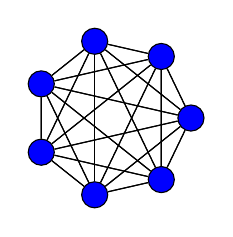
\begin{tikzpicture}
        \foreach \i in {1,...,7}
        {
          \node[defaultNode,fill=blue] (node\i) at ({(360/7)*\i}:1cm) {};
        }
        \foreach \i in {1,...,7}
        {
          \foreach \j in {1,...,7}
          {
            \draw (node\i) -- (node\j);
          }
        }
      \end{tikzpicture}
    \end{center}
  \end{minipage}
  }
  \\
  k-regular Graph
  & {A graph where $\forall v \in V, d(v) = k$ or $\forall v \in V, d^+(v) = d^-(v) = k$.
    \medskip
    
    \begin{minipage}[t]{\linewidth}
      \begin{center}
        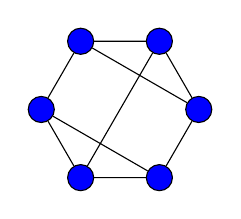
\begin{tikzpicture}
          \node[defaultNode,fill=blue] (A) at (0:1cm) {};
          \node[defaultNode,fill=blue] (B) at (60:1cm) {};
          \node[defaultNode,fill=blue] (C) at (120:1cm) {};
          \node[defaultNode,fill=blue] (D) at (180:1cm) {};
          \node[defaultNode,fill=blue] (E) at (240:1cm) {};
          \node[defaultNode,fill=blue] (F) at (300:1cm) {};

          \draw
          (A) -- (B)
          (A) -- (C)
          (B) -- (C)
          (C) -- (D)
          (D) -- (E)
          (D) -- (F)
          (E) -- (F)
          (F) -- (A)
          (B) -- (E)
          ;
        \end{tikzpicture}
      \end{center}
    \end{minipage}
  }
  \\
  Bipartite Graph
  & {A graph $G = (V,E)$ is bipartite $\iff$ $\exists V', V'' \subset V ~s.t.$ $\forall e \in E, e_1 \in V' \land e_2 \in V''$. This equates to the graph not having any odd-length cycles.
    \medskip

    \begin{minipage}[t]{\linewidth}
      \begin{center}
        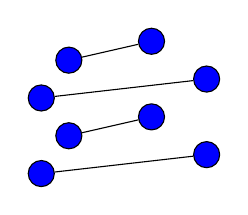
\begin{tikzpicture}

          \node[defaultNode,fill=blue] (node0) at (0.0,0.0) {} ;
          \node[defaultNode,fill=blue] (node1) at (2.1,0.24) {} ;
          \node[defaultNode,fill=blue] (node2) at (0.35,0.48) {} ;
          \node[defaultNode,fill=blue] (node3) at (1.4,0.72) {} ;
          \node[defaultNode,fill=blue] (node4) at (0.0,0.96) {} ;
          \node[defaultNode,fill=blue] (node5) at (2.1,1.2) {} ;
          \node[defaultNode,fill=blue] (node6) at (0.35,1.44) {} ;
          \node[defaultNode,fill=blue] (node7) at (1.4,1.68) {} ;

          \draw
            (node0) -- (node1)
            (node2) -- (node3)
            (node4) -- (node5)
            (node6) -- (node7)
            ;

        \end{tikzpicture}
      \end{center}
    \end{minipage}
  }

\end{longtblr}


\end{document}
